\chapter{Graph and Subgraph Isomorphism}

Rishnak eagerly searched for Ajur because he wanted to share more new concepts with him. It did not take long for Rishnak to find Ajur and Jura walking along the bank of a (presumably haunted) pond in the cemetery. Rishnak immediately started the session with a small variant on what they had already been discussing.

Rishnak said, ``A graph whose vertices are labeled is called a \textit{labeled graph}, while one without labels for vertices is called an \textit{unlabeled graph}. Two labeled graphs are equivalent if they are identical, for example these two graphs''---he flashed his hands to form a pair of labeled graphs in the air in front of Ajur [Figure~\ref{8g1}] [Figure~\ref{8g11}]---``are equivalent.''

Ajur studied the two graphs for a moment, then nodded.

Rishnak waved his hands again and a third graph appeared [Figure~\ref{8g2}].  ``This third graph is not equivalent to the other two graphs because there is no longer an edge between vertices~1 and~2 or between vertices~3 and~4. Or you could say that the vertex labels are different.''

\begin{figure}
\begin{center}
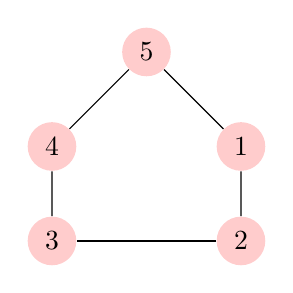
\begin{tikzpicture}
  [scale=.6,auto=left,every node/.style={circle,fill=red!20}]
  \node (n1) at (5,5) {1};
  \node (n4) at (1,5)  {4};
  \node (n3) at  (1,3) {3};
  \node (n2) at (5,3)  {2};
  \node (n5) at (3,7)  {5};

  \foreach \from/\to in {n1/n2,n2/n3,n3/n4,n4/n5,n1/n5}
    \draw (\from) -- (\to);

\end{tikzpicture}
\caption{A labeled graph with five vertices and five edges}\label{8g1}
\end{center}

\end{figure}
\begin{figure}
\begin{center}
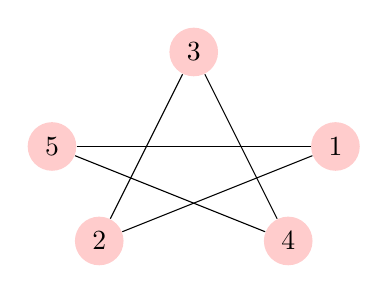
\begin{tikzpicture}
  [scale=.6,auto=left,every node/.style={circle,fill=red!20}]
   \node (n1) at (6,5) {1};
  \node (n5) at (0,5)  {5};
  \node (n2) at  (1,3) {2};
  \node (n4) at (5,3)  {4};
  \node (n3) at (3,7)  {3};

  \foreach \from/\to in {n1/n2,n2/n3,n3/n4,n4/n5,n5/n1}
    \draw (\from) -- (\to);

\end{tikzpicture}
\caption{A second labeled graph with five vertices and five edges that is equivalent to the graph shown in Figure~\ref{8g1}}\label{8g11}
\end{center}
\end{figure}

\begin{figure}
\begin{center}
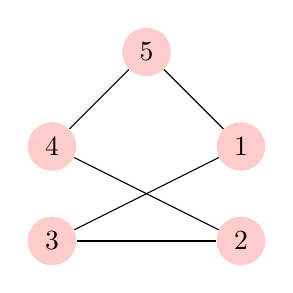
\begin{tikzpicture}
  [scale=.6,auto=left,every node/.style={circle,fill=red!20}]
   \node (n1) at (5,5) {1};
  \node (n4) at (1,5)  {4};
  \node (n3) at  (1,3) {3};
  \node (n2) at (5,3)  {2};
  \node (n5) at (3,7)  {5};


  \foreach \from/\to in {n1/n3,n2/n4,n3/n2,n1/n5,n5/n4}
    \draw (\from) -- (\to);

\end{tikzpicture}
\caption{A third labeled graph with five vertices and five edges that is not equivalent to the graphs shown in Figure~\ref{8g1} and Figure~\ref{8g11} because the vertex labels are differ from that of either of the two other graphs}\label{8g2}
\end{center}
\end{figure}

Ajur said ``I see the differences, but when are two graphs the same?''

Rishnak smiled and said, ``Good question. Two graphs are called \textit{isomorphic}---meaning structurally the same---if they are equivalent under a vertex relabeling. For example, if in the third graph [Figure~\ref{8g2}], vertex~2 is relabeled as vertex~3 and similarly vertex~3 is relabeled as vertex~2, then the third graph becomes equivalent or isomorphic to the other two graphs.''

Ajur studied the third graph again and said, ``Aha, I see.''

Rishnak continued, ``We can also say that if a graph~$G$ is equivalent to a graph~$H$, and~$H$ is equivalent to another graph~$M$, then $G$ is equivalent to graph~$M$. In other words, the relation of graphs being  equivalent or isomorphic is \textit{transitive}. And to test whether two graphs are isomorphic is actually a very hard problem, though it is not as hard as finding a Hamiltonian cycle in a graph.''

Ajur thought about this. If two graphs are isomorphic, they should have the same number of vertices, the same number of edges, the same degree sequences, the same length for the longest cycle, the same length for the shortest cycle, and so on. He repeated these to Rishnak, then asked, ``Can we use some of these properties to show to graphs are isomorphic?''

Rishnak furled his brow and said, ``Unfortunately not. These properties of graphs are called \textit{graph invariants}, but by no mean are these invariants exhaustive. We do not know of a single easily computable invariant that can be used to test whether or not two given graphs are isomorphic.''

Ajur frowned at this, frustrated that there were unsolved problems like this.

Rishnak said, ``It is much easier to detect that two graphs are not isomorphic. Can you draw two graphs with the same number of vertices and the same number of edges that are not isomorphic?''

Ajur thought a bit then grabbed a stick and drew two graphs in the dirt [Figure~\ref{8g3}] [Figure~\ref{8g4}]. He said, ``Both these graphs have six vertices and nine edges, but the first graph is bipartite---we know this because all cycles are of even length---while the other graph is not bipartite because it has a cycle of length~3. Therefore, these two graphs are not isomorphic.''

Rishnak smiled.

\begin{figure}
\begin{center}
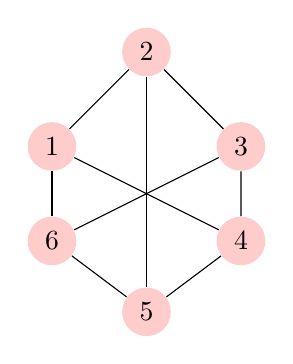
\begin{tikzpicture}
  [scale=.3,auto=left,every node/.style={circle,fill=red!20}]
  \node (n1) at (1,7) {1};
  \node (n2) at (5,11)  {2};
  \node (n3) at (9,7)  {3};
  \node (n4) at (9,3) {4};
  \node (n5) at (5,0)  {5};
  \node (n6) at (1,3) {6};
  
   \foreach \from/\to in {n1/n2,n2/n3,n3/n4,n4/n5,n5/n6,n1/n6,
  n2/n5, n6/n3,n1/n4}
    \draw (\from) -- (\to);
    \end{tikzpicture}
\caption{A bipartite graph with six vertices and nine edges}\label{8g3}
\end{center}
\end{figure}

\begin{figure}
\begin{center}
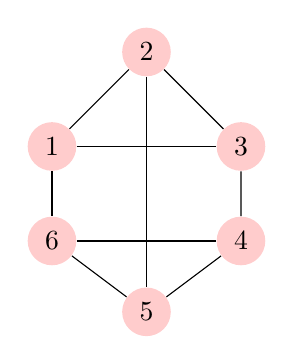
\begin{tikzpicture}
  [scale=.3,auto=left,every node/.style={circle,fill=red!20}]
  \node (n1) at (1,7) {1};
  \node (n2) at (5,11)  {2};
  \node (n3) at (9,7)  {3};
  \node (n4) at (9,3) {4};
  \node (n5) at (5,0)  {5};
  \node (n6) at (1,3) {6};
  
   \foreach \from/\to in {n1/n2,n2/n3,n3/n4,n4/n5,n5/n6,n1/n6,
  n2/n5, n6/n4,n1/n3}
    \draw (\from) -- (\to);
    \end{tikzpicture}
\caption{A non-bipartite graph with six vertices and nine edges}\label{8g4}
\end{center}
\end{figure}

Ajur thought for awhile, then said that partial solutions to the graph isomorphism problem would be very useful if you wanted to test whether a given graph is in a collection of graphs, a problem that comes up in chemistry.

Rishnak was pleased that Ajur was thinking about some of the practical applications of graph theory. Rishnak said, ``There is an easier method to test for isomorphism between two rooted trees. Let's start with how we can encode a labeled tree. We'll use an approach called a Pr\"ufer code. The construction is iterative, and the Pr\"ufer code of a labeled tree with~$n$ vertices is a code of length~$n-2$. Here's the algorithm, but first, remember that a leaf of a tree is a vertex that is connected to only one other vertex.

\begin{enumerate}
\item Let Pr{\"u}fer code~$P_c$ be an empty string.

\item Find leaf vertex~$v$ with the smallest label, then identify vertex~$w$ that connects vertex~$v$ to the rest of tree.

\item Remove~$v$ from the tree and append~$w$ to Pr{\"u}fer code~$P_c$.

\item Repeat from step~2 until we are left with only two vertices.''
\end{enumerate}

Ajur raised his eyebrows and said, ``Wow, that's a lot to take in.''

Rishnak laughed and said, ``Try it on this rooted tree.''  He waved his hands and a new graph [Figure~\ref{8g5}] appeared in front of Ajur.

Ajur took a deep breath and said, ``Okay, the smallest leaf is vertex~4. Its adjacent vertex is labeled~2, so we append~2 to Pr\"ufer code~$P_c$ and remove vertex~4. The next smallest leaf vertex is labeled~5 and is adjacent to vertex~2. Therefore, we append~2 to~$P_c$ and remove vertex~5. Now vertex~2 is the smallest leaf vertex and its adjacent vertex is vertex~1, so we append~1 to $P_c$ and remove vertex~2. At this point, $P_c$ is~$221$, but we're not done yet.''

Rishnak smiled and said, ``Right, go on.''

Ajur said, ``Wait, vertex~1 is now the smallest leaf vertex, but it was originally the root of the tree. Is that okay?''

Rishnak said, ``Yes, that's part of the algorithm.''

Ajur shrugged and continued, ``Okay, vertex~1 is next and its adjacent vertex is vertex~3, so vertex~1 is removed and we append~3 to $P_c$. The next smallest leaf is then vertex~6 and its adjacent vertex is vertex~3, so we again append~3 to~$P_c$. We stop when there are only two vertices left, so we are done. The Pr{\"u}fer code for the tree is $P_c=22133$.''

Rishnak nodded and said, ``Good, since the length of~$P_c$ is~5, we can immediately conclude that there are seven vertices in the tree. Further, we can also conclude that vertices labeled~4, 5, 6, and~7 are the leaf vertices since they do not appear in the given Pr\"ufer code.''

\begin{figure}
\begin{center}

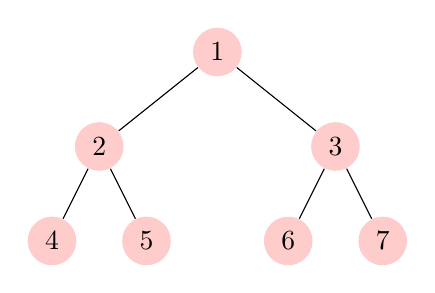
\begin{tikzpicture}
  [scale=.6,auto=left,every node/.style={circle,fill=red!20}]
  \node (n1) at (5.5,7) {1};
  \node (n2) at (3,5)  {2};
  \node (n3) at (8,5)  {3};
  \node (n4) at (2,3) {4};
  \node (n5) at (4,3)  {5};
  \node (n6) at (7,3)  {6};
  \node (n7) at (9,3)  {7};

  \foreach \from/\to in {n1/n2,n1/n3,n2/n4,n2/n5,n3/n6,n3/n7}
    \draw (\from) -- (\to);

\end{tikzpicture}

\caption{A rooted tree with seven vertices, of which four vertices are leaf vertices}\label{8g5}
\end{center}
\end{figure}

Ajur asked, ``What about unlabeled trees? Can we find a Pr\"ufer code for an unlabeled tree?''

Rishnak replied with a resounding yes and explained the steps to follow for a rooted tree. He said, ``For any tree, one needs to first choose an appropriate root vertex, which we can call the \textit{center} of the tree. Here's the basic algorithm to follow.
%\textbf{Raju: be careful, not every tree has a center which is a vertex!}} 
\begin{enumerate}
    \item Assign each leaf vertex a label of~01.
    \item Let~$x$ be a non-leaf vertex. For all of the children of~$x$, sort these labels in order. Assign vertex~$x$ with a label that is a~0, followed by the concatenation of the sorted labels of its children, followed by a~1.
    \item Repeat step 2 until you label the root vertex.''
\end{enumerate}

Rishnak knew this was a lot to follow. He said, ``Have another look at this tree [Figure~\ref{8g5}]. If this was an unlabeled graph, then leaf vertices~4, 5, 6, and~7 would all be labeled~01. Then vertex~2 would be labeled~$001011$. Same with vertex~3. Finally, root vertex~1 would have the label~$000101100101111$, which would serve as the Pr\"ufer code for this tree.''

Ajur tried his best to follow. After some time, he said, ``I think I see. Using these Pr\"ufer codes, we could compare them to see if they match, which would show that the two rooted trees are the same---I mean, isomorphic.''

Rishnak smiled and said, ``Precisely. And closely related to the problem of graph isomorphism is a problem that has plenty of uses in real life, not just in the ghoulish realm.''

Ajur chuckled at the bad joke.

Rishnak continued, ``Instead of asking whether two graphs are structurally the same and therefore isomorphic, given two graphs~$G$ and~$H$, the \textit{subgraph isomorphism} problem is to determine whether there is a subgraph of~$G$ that is isomorphic to~$H$.''

Ajur said, ``A subgraph of~$G$. I understand. This approach could be used to test whether graph~$G$ with~$n$ vertices has a Hamiltonian cycle by choosing graph~$H$ to be a cycle of length~$n$ and asking whether there is a subgraph of~$G$ isomorphic to~$H$.''

Rishnak nodded and said, ``Yes, and that is the reason why the subgraph isomorphism problem is hard. On the other hand, if both~$G$ and~$H$ are labeled graphs, there are heuristics to test whether~$H$ occurs in~$G$ as a subgraph. This type of labeled subgraph isomorphism problem has many applications in medical imaging and chemical structure identification.''

Ajur marveled at how connected and useful graphs and subgraphs were.

\subsection*{Question for the sixth day}
Rishnak said, ``Okay, Ajur, the time has come. Here is the question for the sixth day. Can you draw a tree with a Pr{\"u}fer code of~232?''

\textit{Before you turn the page, try to come up with an answer of your own!}

\newpage
\subsection*{Answer for the sixth day}
Ajur nodded and said, ``Yes, first of all, I know that this will be a tree with five vertices because the Pr\"ufer code has a length of~3.''

Without hesitating, Ajur drew a tree in the dirt [Figure~\ref{6q1}].  He said, ``This is the tree.''

\begin{figure}
\begin{center}

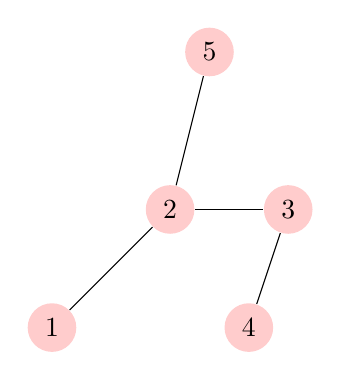
\begin{tikzpicture}
  [scale=.5,auto=left,every node/.style={circle,fill=red!20}]
  \node (n1) at (0,0) {1};
  \node (n2) at (3,3)  {2};
  \node (n3) at (6,3)  {3};
  \node (n4) at (5,0) {4};
  \node (n5) at (4,7)  {5};
 

  \foreach \from/\to in {n1/n2,n4/n3,n2/n3,n2/n5}
    \draw (\from) -- (\to);

\end{tikzpicture}

\caption{Tree with 5 vertices with a Pr\"ufer code of~232}\label{6q1}
\end{center}
\end{figure}

Rishnak was happy with Ajur's answer, and Ajur was eager to go home, with Jura at his side, to think about all of the applications graphs and subgraphs might have in the world.
